\chapter{Τεχνικές λεπτομέρειες}
\label{chap7}

\section{Εισαγωγή}
\label{chap7_Intro}

Για τη μοντελοποίηση και της αξιολόγηση της τεχνικής χρησιμοποιήθηκαν τα τρία βασικά εργαλεία \matlabR, \gem και \mcpat, όπως παρουσιάζονται στο Σχήμα \ref{fig:chap7_simulation_tools}. Αρχικά στο \matlab υλοποιήθηκε η μοντελοποίηση των σφαλμάτων καθώς και οι διαφορετικές εκδοχές της προτεινόμενης τεχνικής λογικής μετάθεσης πλαισίων. Στη συνέχεια έγινε η εισαγωγή των χαρτών σφαλμάτων που παρήχθησαν από το \matlab στο \gem, ώστε να πραγματοποιηθεί η εξομοίωση λειτουργίας ενός επεξεργαστή όταν υπάρχουν σφάλματα στη Μονάδα Δυναμικής Πρόβλεψης Διακλαδώσεων. Για την εξαγωγή αποτελεσμάτων εκτελέστηκαν αντιπροσωπευτικά τμήματα των μετροπρογραμμάτων \spec. Τέλος, χρησιμοποιήθηκε το εργαλείο \mcpat έχοντας ως είσοδο τα αποτελέσματα της εξομοίωσης του \gem, ώστε να γίνει ο υπολογισμός της συνολικής καταναλωμένης ενέργειας πριν και μετά την εφαρμογή των προτεινόμενων μοντέλων.

\begin{figure}[h]
    \centering
    \fbox{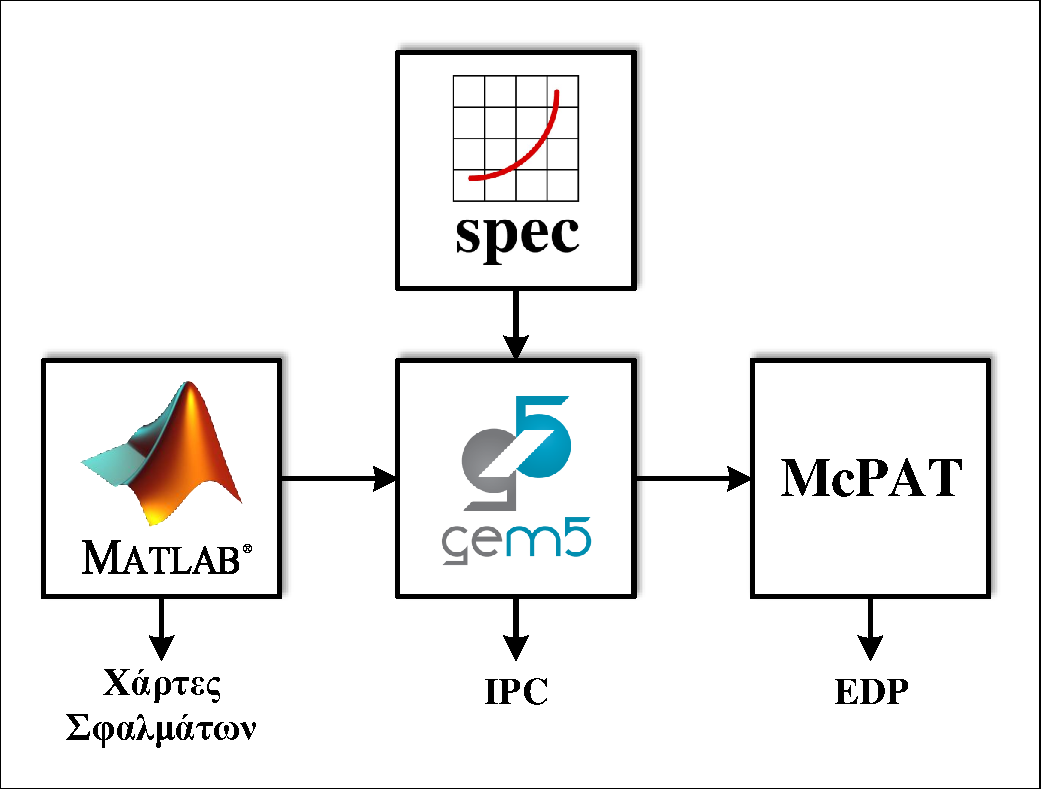
\includegraphics[width=0.7\linewidth, trim=0.5cm 0.6cm 0.5cm 0.8cm, clip=true]{\simulationsDIR/chap7_simulation_stages.pdf}}
    \caption{Ακολουθία πειραματικής αξιολόγησης}
    \label{fig:chap7_simulation_tools}
\end{figure}

%----------------------------------------------------------%

\section{\matlab}
\label{chap7_matlab}

Η μοντελοποίηση των ελαττωματικών κυψελίδων της μνήμης καθώς μειώνεται η τάση λειτουργίας και επομένως αυξάνεται η πιθανότητα σφάλματος, πραγματοποιήθηκε μέσω του εργαλείου \matlabR της \en{MathWorks} (\en{\url{https://www.mathworks.com/products/matlab.html}}), το οποίο περιέχει τις κατάλληλες συναρτήσεις ώστε τα σφάλματα να τοποθετούνται τυχαία στα δυαδικά ψηφία της μνήμης. Η προτεινόμενη τεχνική της λογικής μετάθεσης πλαισίων υλοποιήθηκε στο συγκεκριμένο εργαλείο ώστε στον εξομοιωτή να δίδεται ώς είσοδος ο αντίστοιχος τροποποιημένος χάρτης. Επομένως, για κάθε παραγόμενο χάρτη σφαλμάτων εξάγονται ταυτόχρονα και οι τροποποιημένοι χάρτες σφαλμάτων κάθε τεχνικής. Ο κώδικας υλοποίησης περιέχεται στο συνοδευτικό οπτικό μέσο αποθήκευσης (\en{CD}) καθώς και στην ηλεκτρονική διεύθυνση \en{\url{https://github.com/filippo-ceid/HSIS_Thesis/}}. Η εκτέλεση του για την παραγωγή Ν χαρτών σφαλμάτων πραγματοποιείται μεσώ της εντολής:

\begin{center}
    \begin{tcolorbox}[width=0.9\linewidth]
        \selectlanguage{english}\ttfamily
        >> fault\_map\_btb\_permutation(N)
    \end{tcolorbox}
\end{center}

Στις πρώτες γραμμές του κώδικα βρίσκονται οι σημαντικότερες μεταβλητές τροποποίησης των εξομοιώσεων ώστε ο χρήστης να μπορεί εύκολα να παράξει χάρτες σφαλμάτων για διαφορετικά μοντέλα, όπως μέγεθος/οργάνωση του Πίνακα Πρόβλεψης Προορισμού Διακλάδωσης, πιθανότητα σφάλματος, πλήθος καταχωρητών ανά τμήμα, χρήση σειριακού ή παράλληλου αλγορίθμου και άλλα.
\par
Στον κώδικα υπάρχουν τρεις καθολικές μεταβλητές η ενεργοποίηση των οποίων προσφέρει επιπλέον δυνατότητες στο χρήστη. Η μεταβλητή $``$\textit{\en{statistics}}$"$ ενεργοποιεί την εκτύπωση στατιστικών για κάθε χάρτη σφαλμάτων που παράγεται. Η μεταβλητή $``$\textit{\en{debugging}}$"$ ενεργοποιεί την παροχή αναλυτικών πληροφοριών κατά την εκτέλεση, ώστε να δίνεται η δυνατότητα στο χρήστης να παρακολουθεί ολόκληρη τη διαδικασία του υπολογισμού κατάλληλων τιμών για τους Καταχωρητές Διαμόρφωσης. Τέλος, η μεταβλητή $``$\textit{\en{export\_fmaps}}$"$ ενεργοποιεί τη δυνατότητα εξαγωγής των παραγόμενων χαρτών σφαλμάτων σε ειδικά διαμορφωμένα αρχεία τα οποία οδηγούνται ώς είσοδο στον εξομοιωτή \gem. Μία τυπική μορφή εξόδου παρουσιάζεται στο Σχήμα \ref{fig:chap7_matlab_output}.

\begin{figure}[!b]
    \centering
    \fbox{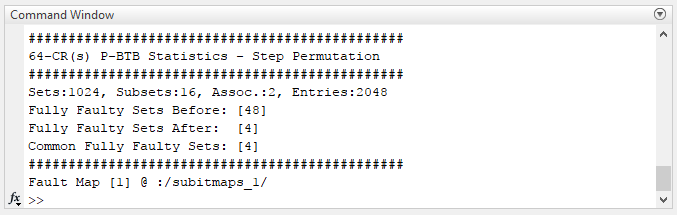
\includegraphics[width=0.85\linewidth, clip=true]{\simulationsDIR/chap7_matlab_output.png}}
    \caption{Έξοδος εκτέλεσης του κώδικα \matlab}
    \label{fig:chap7_matlab_output}
\end{figure}

%----------------------------------------------------------%

\section{\gem}
\label{chap7_gem5}

Όπως προαναφέρθηκε, οι εξομοιώσεις σε επίπεδο εκτέλεσης εντολών εκτελέστηκαν με τη χρήση του εξομοιωτή αρχιτεκτονικής υπολογιστών \gem. Ο εξομοιωτής αυτός αποτελεί ένα πολύ ισχυρό εργαλείο ανοικτού κώδικα, το οποίο προσφέρει ποικίλες δυνατότητες με μεγάλη ευελιξία στην τροποποίησή του.
\par
Ο συγκεκριμένος εξομοιωτής αποτελεί ένα συνδυασμό των προγενέστερων εξομοιωτών \en{m5} και \en{gems}, από τα οποία αποκομίστηκαν τα καλύτερα χαρακτηριστικά τους και συνενώθηκαν ώστε να δημιουργηθεί αυτό το πολύ ισχυρό εργαλείο. Από τον εξομοιωτή \en{m5} χρησιμοποιούνται στοιχεία όπως τα πρότυπα κεντρικών μονάδων επεξεργασίας, οι αρχιτεκτονικές συνόλου εντολών, οι μονάδες εισόδου/εξόδου, καθώς και η υποδομή του. Από τον \en{gems} χρησιμοποιούνται στοιχεία όπως τα πρωτόκολλα συνέπειας της κρυφής μνήμης και τα μοντέλα διασύνδεσης. Επιπλέον, έχουν προστεθεί και νέα χαρακτηριστικά, όπως η υποστήριξη στις επικρατέστερες αρχιτεκτονικές συνόλου εντολών \en{ARM} και \en{x86}. Τέλος, αξίζει να αναφερθεί πως οι βασικές γλώσσες προγραμματισμού που το αποτελούν είναι η \en{C++} και η \en{Python}. Για αναλυτικές πληροφορίες παροτρύνεται η μελέτη του \cite{binkert2011gem5}. Τόσο ο πηγαίος κώδικας όσο και επιπρόσθετο υλικό παρέχονται ελεύθερα μέσω της επίσημης ηλεκτρονικής σελίδας του εξομοιωτή (\en{\url{http://gem5.org/}}).
\par
Για τους σκοπούς της παρούσας διπλωματικής εργασίας έγιναν οι κατάλληλες τροποποιήσεις ώστε να προστεθεί η δυνατότητα ανάγνωσης των χαρτών σφαλμάτων, τόσο του Πίνακα Πρόβλεψης Διακλάδωσης όσο και του Πίνακα Πρόβλεψης Προορισμού Διακλάδωσης. Επιπλέον, προστέθηκε η δυνατότητα απενεργοποίησης των ελαττωματικών πλαισίων του Πίνακα Πρόβλεψης Προορισμού Διακλάδωσης. Η διαδικασία εγκατάστασης και εκτέλεσης του τροποποιημένου εξομοιωτή είναι η ακόλουθη:

\begin{center}
    \begin{tcolorbox}[width=\linewidth]
        \selectlanguage{english}\ttfamily
        \fullcomment{\gr{Διαδικασία εγκατάστασης}} \\
        
        \linecomment{\gr{Εγκατάσταση προαπαιτούμενων πακέτων σε} Debian-based \gr{λειτουργικό}} \\
        \$ sudo apt-get install build-essential ssh git zip gcc g++ parallel mercurial scons swig swig3.0 m4 python python-dev libgoogle-perftools-dev zlib1g-dev protobuf-compiler libprotobuf-dev \\
        
        \linecomment{\gr{Λήψη εξομοιωτή}}\\
        \$ git clone \text{git@pc-tca1.ceid.upatras.gr}:/home/git/gem5\_btb \\
        
        \linecomment{\gr{Δήλωση μονοπατιού του εργαλείου} SWIG \gr{και του εξομοιωτή} \gem} \\
        \$ echo "export SWIG=/usr/bin/swig3.0" >{}> $\sim$/.bashrc \\
        \$ echo "export M5\_PATH=/home/<path>/gem5\_btb/" >{}> $\sim$/.bashrc \\
        \linecomment{\gr{Εφαρμογή των δηλωμένων μονοπατιών}} \\
        \$ source $\sim$/.bashrc
    \end{tcolorbox}
\end{center}

\begin{center}
    \begin{tcolorbox}[width=\linewidth]
        \selectlanguage{english}\ttfamily
        \fullcomment{\gr{Διαδικασία δημιουργίας επεξεργαστή και εκτέλεσης εξομοιώσεων}} \\
        
        \linecomment{\gr{Μεταφορά στο σημείο εγκατάστασης του εξομοιωτή}} \\
        \$ cd \$M5\_PATH \\
         
        \linecomment{\gr{Δημιουργία βασικού μοντέλου εξομοιούμενου επεξεργαστή}}\\
        \$ scons build/X86/gem5.opt -j<threads> \\
        
        \linecomment{\gr{Αρχείο παραμετροποίησης του εξομοιούμενου επεξεργαστή}} \\
        \$ ./configs/resize/ntlc\_config.py \\
        \linecomment{\gr{Αρχείο παραμετροποίησης της Μονάδας Πρόβλεψης Διακλαδώσεων}} \\
        \$ ./src/cpu/pred/BranchPredictor.py \\
        
        \linecomment{\gr{Εκτέλεση απλού παραδείγματος εξομοίωσης}} \\
        \$ ./build/X86/gem5.opt --outdir ./BTB\_results/ -i configs/resize/ntlc\_sim.py --profile-cpt=<used\_chechpoints\_path> --batch --medium-cpu --sim-window=<committed\_inst> --atomic-warmup=<warmup\_inst> \\
        
        \linecomment{\gr{Καθαρισμός εξομοιωτή}} \\
        \$ scons -c \\
        
        \fullcomment{\gr{Διαδικασία πραγματοποίησης πολλαπλών πειραμάτων}} \\
        
        \linecomment{\gr{Χρήση ενσωματωμένων χαρτών σφαλμάτων}} \\
        \$ cd src/cpu/pred/ \\
        
        \linecomment{\gr{Χάρτες σφαλμάτων του Πίνακα Πρόβλεψης Διακλάδωσης}} \\
        \$ unzip subitmaps\_BPU\_100fmaps\_choiceCtrs.zip \\
        \$ unzip subitmaps\_BPU\_100fmaps\_globalCtrs.zip \\
        \$ unzip subitmaps\_BPU\_100fmaps\_localCtrs.zip \\
        \$ unzip subitmaps\_BPU\_100fmaps\_localHistoryTable.zip \\
        
        \linecomment{\gr{Χάρτες σφαλμάτων του Πίνακα Πρόβλεψης Προορισμού Διακλάδωσης}} \\
        \$ unzip subitmaps\_BTB\_100fmaps\_serial.zip \\
        \$ unzip subitmaps\_BTB\_100fmaps\_parallel.zip \\
        
        \linecomment{\gr{Τοποθέτηση νέου συνόλου χαρτών σφαλμάτων}} \\
        \$ cp -r <path>/subitmaps\_<...> \$M5\_PATH/src/cpu/pred/
    \end{tcolorbox}
\end{center}

\begin{center}
    \begin{tcolorbox}[width=\linewidth]
        \selectlanguage{english}\ttfamily
        \linecomment{\gr{Εκτέλεση κώδικα εξομοίωσης (απαιτείται τροποποίηση)}} \\
        \linecomment{\gr{(δήλωση χαρτών σφαλμάτων, πλήθους εξομοιώσεων,} chechpoint \gr{κ.α.)}} \\
        
        \linecomment{\gr{Εξομοιώσεις σφαλμάτων στον Πίνακα Πρόβλεψης Διακλάδωσης}} \\
        \$ ./run-gem5\_predictor\_parallel.sh \\
        \linecomment{\gr{Εξομοιώσεις σφαλμάτων στον Πίνακα Πρόβλεψης Προορισμού Διακλάδωσης}} \\
        \$ ./run-gem5\_parallel.sh \\
        
        \linecomment{\gr{Συγκέντρωσης αποτελεσμάτων}} \\
        \$ ./BTB\_results/gem5\_to\_csv\_core\_stats\_<clean/faulty>.sh \\
        \$ ./BTB\_results/gem5\_to\_csv\_predictor\_stats\_<clean/faulty>.sh
    \end{tcolorbox}
\end{center}

Περαιτέρω πληροφορίες διατίθενται στα σχετικά αρχεία οδηγιών \textlatin{HOW\_TO\_SETUP.txt} και \textlatin{HOW\_TO\_RUN.txt}. Για τη λήψη της τροποποιημένης έκδοσης απαιτείται η επικοινωνία στην ηλεκτρονική διεύθυνση \en{\email} ώστε να παραληφθούν οι απαραίτητοι κωδικοί πρόσβασης. Η δυνατότητα εκτέλεσης των μετροπρογραμμάτων \spec προϋποθέτει την αγορά της σχετικής άδεια από το χρήστη (\en{\url{https://www.spec.org/cpu2006/}}). Αναλυτικές πληροφορίες για τα μετροπρογράμματα που χρησιμοποιήθηκαν βρίσκονται στο \cite{henning2006spec}. Μία τυπική μορφή εξόδου ολοκληρωμένης εξομοίωσης παρουσιάζεται στο Σχήμα \ref{fig:chap7_gem5_output}.

\begin{figure}[h]
    \centering
    \fbox{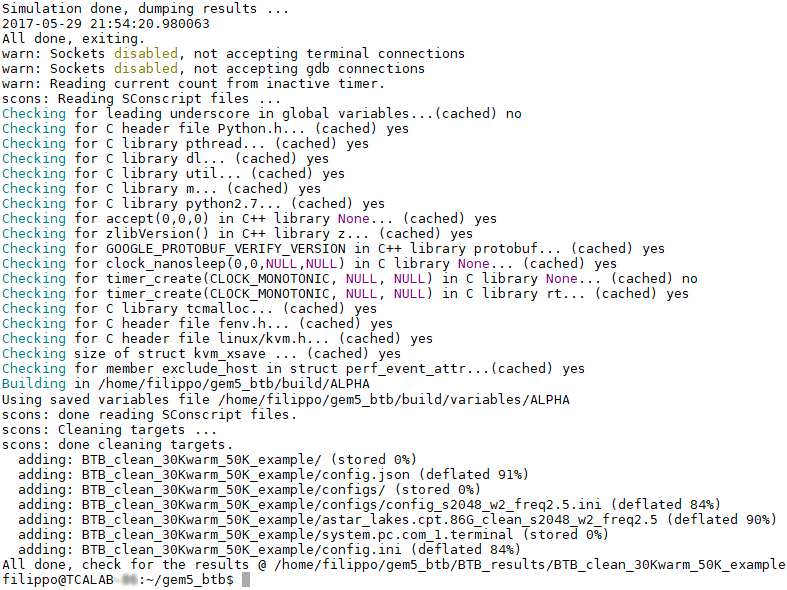
\includegraphics[width=0.85\linewidth, clip=true]{\simulationsDIR/chap7_gem5_output.png}}
    \caption{Έξοδος ολοκλήρωσης εκτέλεσης \gem}
    \label{fig:chap7_gem5_output}
\end{figure}

%----------------------------------------------------------%

\section{\mcpat}
\label{chap7_mcpat}

Για την εξαγωγή αποτελεσμάτων κατανάλωσης, επιφάνειας και χρόνου χρησιμοποιήθηκε το αναγνωρισμένο εργαλείο \mcpat (έκδοση 1.3) ανοικτού κώδικα, το οποίο παρέχει αρκετά ακριβείς υπολογισμού σε σχεδιασμούς πολυπύρηνων συστημάτων διαφορετικών αρχιτεκτονικών. Διαθέτει μοντέλα εξομοίωσης τεχνολογίας από 90\nm έως 20\nm και για την μοντελοποίηση των κομματιών μνήμης χρησιμοποιεί το εργαλεία \cacti, το οποίο τροποποιήθηκε κατάλληλα ώστε να ενσωματωθεί η διάσπαση του Πίνακα Πρόβλεψης Προορισμού Διακλάδωσης για την υλοποίηση της προτεινόμενης τεχνικής. Περισσότερες πληροφορίες για τα δύο εργαλεία βρίσκονται στα \cite{li2009mcpat} και \cite{li2009mcpat} αντίστοιχα.
\par
Τόσο ο πηγαίος κώδικας όσο και επιπρόσθετο υλικό των εργαλείων διατίθενται ελεύθερα στην ηλεκτρονική σελίδα της \en{Hewlett-Packard Development Company, L.P.} (\en{\url{http://www.hpl.hp.com/research/mcpat/}} και \en{\url{http://www.hpl.hp.com/research/cacti/}}). Η τροποποιημένη έκδοση του εργαλείου παρέχεται με τον εξομοιωτή \gem και η διαδικασία εκτέλεσης του είναι η ακόλουθη:

\begin{center}
    \begin{tcolorbox}[width=\linewidth]
        \selectlanguage{english}\ttfamily
        \linecomment{\gr{Εγκατάσταση προαπαιτούμενων πακέτων σε} Debian-based \gr{λειτουργικό}} \\
        \$ sudo apt-get install libc6-dev-i386 g++-multilib \\
        
        \linecomment{\gr{Μεταφορά στο σημείο εγκατάστασης}} \\
        \$ cd \$M5\_PATH/hw\_analysis/mcpat/ \\
        
        \linecomment{\gr{Αρχείο δήλωσης ελάχιστων διασπάσεων της μνήμης (γραμμές 42 έως 44)}} \\
        \linecomment{\gr{(προεπιλεγμένα δεν καθορίζεται όριο από το χρήστη)}} \\
        \$ ./mcpat\_source/array.cc \\
        
        \linecomment{\gr{Εκτέλεση απλού παραδείγματος}} \\
        \linecomment{\gr{Μετατροπή των αποτελεσμάτων του} \gem \gr{σε αρχείο τύπου} XML} \\
        \$ perl m5-mcpat.pl stats.txt config.ini mcpat-template.xml > output.xml \\
        \linecomment{\gr{Εκτέλεση υπολογισμών με παράμετρο εισόδου το αρχείο} XML} \\
        \$ ./mcpat\_source/mcpat -infile output.xml -print\_level <level of details 0-5>  > mcpat\_results.txt \\
        
        \linecomment{\gr{Κώδικας πολλαπλών υπολογισμών (απαιτείται τροποποίηση)}} \\
        \linecomment{\gr{(δήλωση μονοπατιού αποτελεσμάτων/παραμέτρων} \gem \gr{κ.α.)}} \\
        \$ ./run-mcpat.sh \\
        
        \linecomment{\gr{Συγκέντρωσης αποτελεσμάτων}} \\
        \$ ./mcpat\_to\_csv\_stats\_<clean/faulty>sh
    \end{tcolorbox}
\end{center}

Στο Σχήμα \ref{fig:chap7_mcpat_output} παρουσιάζεται μία τυπική μορφή εξόδου από την εκτέλεση του κώδικα πολλαπλών υπολογισμών, ενώ στο Σχήμα \ref{fig:chap7_mcpat_results_output} δίδεται ένα τμήμα του αρχείου εξόδου της εκτέλεση, στο οποίο διακρίνεται η κατανάλωση του επεξεργαστή για την εκτέλεση του παραδείγματος.

\begin{figure}[h]
    \centering
    \fbox{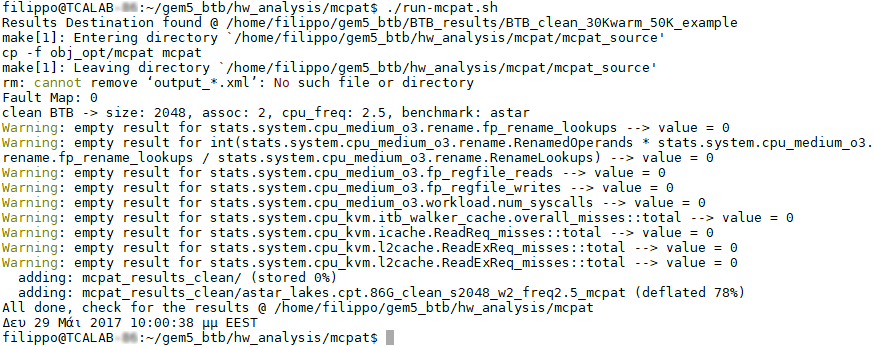
\includegraphics[width=0.82\linewidth, clip=true]{\simulationsDIR/chap7_mcpat_output.png}}
    \caption{Έξοδος ολοκλήρωσης εκτέλεσης \mcpat}
    \label{fig:chap7_mcpat_output}
\end{figure}

\begin{figure}[h]
    \centering
    \fbox{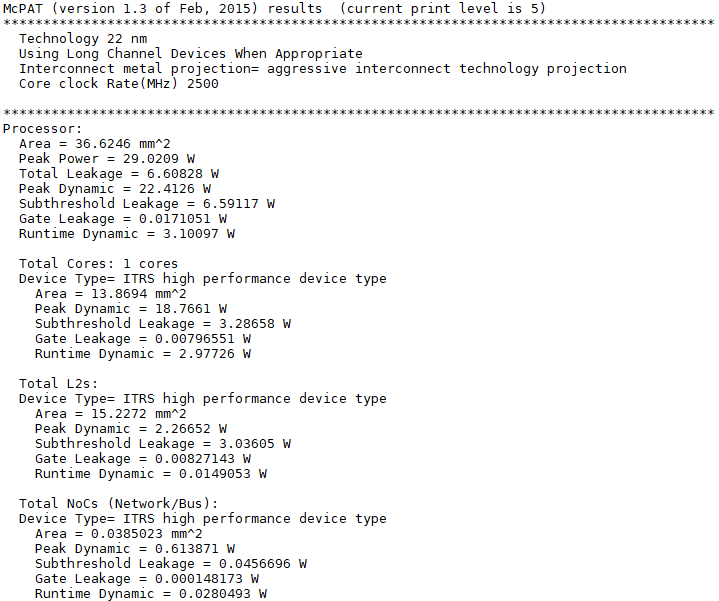
\includegraphics[width=0.82\linewidth, clip=true]{\simulationsDIR/chap7_mcpat_results_file.png}}
    \caption{Αποτελέσματα κατανάλωσης για την εκτέλεση του παραδείγματος}
    \label{fig:chap7_mcpat_results_output}
\end{figure}

%----------------------------------------------------------%
